\documentclass[10pt,a4paper]{article} %#Establece el tipo de documento y sus especificaciones
%##Lista de paquetes que se podrán usar en el documento
\usepackage[left=2cm,right=2cm,top=2cm,bottom=2cm]{geometry}
\usepackage[dvipsnames]{xcolor}
\usepackage[fleqn]{mathtools}
\usepackage{booktabs}
\usepackage{amsmath}
\usepackage{latexsym}
\usepackage{graphicx}%##Paquete para llamar imagenes
\usepackage{nccmath}
\usepackage{multicol}
\usepackage{listings}
\usepackage{tasks}
\usepackage{color}
\usepackage{float}
\usepackage{lipsum}
\usepackage[spanish]{babel}
\UseRawInputEncoding

\definecolor{colorIPN}{rgb}{0.5, 0.0,0.13}
\definecolor{colorESCOM}{rgb}{0.0, 0.5,1.0}
\graphicspath{ {imagenes/} }

\begin{document} %##Indica donde inicia el documento
	%#########################################################
	\begin{titlepage}
		\centering
		{ \huge \bfseries \color{colorIPN}{Instituto Politécnico Nacional} \par}
		{ \Large \bfseries  \color{colorESCOM}{Escuela Superior de C{\' o}mputo} \par }
		\vspace{1cm}%##Inserta una separación de tamaño exacto entre líneas
		{\huge\Large \color{colorIPN}{Web App Development}.\par}
		\vspace{1.5cm}
		{\huge\Large  \color{colorESCOM}{Ejercicio 4 : Instalar Heroku CLI}\par}
		\vspace{2cm}
		{\Large\itshape \color{colorIPN}{Profesor: M. en C. Jos{\' e} Asunci{\' o}n Enr{\' i}quez Z{\' a}rate}\par} \hfill \break
		\vspace{2cm}
		{\Large\itshape \color{colorIPN}{Alumno: Mauro Sampayo Hern{\' a}ndez}\par} \hfill \break
		{\Large\itshape \color{colorIPN}{mauro\_luigi@hotmail.com}\par} \hfill \break
		{\Large\itshape \color{colorIPN}{3CM18} \par}
		\vfill
		{\large \color{colorIPN}{\today}\par} 
		\vfill
	\end{titlepage}
	
	\renewcommand\lstlistingname{Quelltext} 
	
	\settasks{
		counter-format=(tsk[r]),
		label-width=4ex
	}
	\tableofcontents 
	\pagebreak
	
	\pagenumbering {arabic} %##Coloca el contador de páginas a 1 y comienza a numerar de acuerdo con el estilo especificado. En este caso dicho estilo de numeracion es el arabigo
	
	\pagebreak
	
	%################################################
	\section{\color{colorIPN}{Introducci{\' o}n}}%##Crea secciones númeradas, en este caso esta es la seccion 1
	{\large Heroku es una plataforma basada en la nube como servicio (PaaS) dise{\~n}ada para que los desarrolladores y equipos creen, env{\'i}en, supervisen y escalen aplicaciones modernas. Esta plataforma brinda a los desarrolladores mayor tiempo para centrarse en el producto principal sin tener que preocuparse de mantener la infraestructura de la aplicaci{\'o}n. 
		
		
		\vspace{0.5cm}
		Heroku adem{\'a}s ofrece herramientas, servicios y flujos de trabajo integrados para ayudar a las organizaciones de todos los tama{\~n}os a maximizar la productividad individual y del equipo para poder entregar aplicaciones en el mercado m{\'a}s r{\'a}pidamente.
		
		\vspace{0.5cm}
		Adicionalmente Heroku cuenta con una interfaz de l{\'i}nea de comando (Heroku CLI por sus siglas en ingl{\'e}s) la cu{\'a}l facilita la creaci{\'o}n y administraci{\'o}n de las aplicaciones que sean desarrolladas por el usuario en esta plataforma y la cu{\'a}l puede ser descargada e instalada. En este reporte se detallar{\'a} el proceso para la instalaci{\'o}n de Heroku CLI.}
	
	%\subsection{ \color{colorESCOM}{Sub Sección 1}} %##Crea subsecciones numeradas
	%\lipsum[2-3] %##Añade tecto lorem ipsum
	
	\pagebreak
	
	%################################################
	\section{\color{colorIPN}{Conceptos}}
	
	\subsection{ \color{colorESCOM}{Inform{\'a}tica en la nube}}
	{\large La inform{\'a}tica en la nube es el suministro de servicios inform{\'a}ticos (incluidos servidores, almacenamiento, bases de datos, redes, software, an{\'a}lisis e inteligencia) a trav{\'e}s de Internet (la nube), cuyo objetivo es ofrecer una innovaci{\'o}n m{\'a}s r{\'a}pida, recursos flexibles y econom{\'i}as de escala.
		
		
		\vspace{0.5cm}
		La mayor{\'i}a de los servicios de inform{\'a}tica en la nube se engloban en cuatro categor{\'i}as generales: infraestructura como servicio (IaaS), plataforma como servicio (PaaS), sin servidor y software como servicio (SaaS).
		
		
		\vspace{0.5cm}
		Existen 3 tipos de nubes inform{\'a}ticas:}
	
	\subsubsection{\color{colorESCOM}{Nubes p{\'u}blicas:}}
	{\large Los recursos en la nube (como los servidores y el almacenamiento) son propiedad de un proveedor de servicios en la nube que los administra y los ofrece a trav{\'e}s de Internet. Con una nube p{\'u}blica, todo el hardware, el software y los dem{\'a}s componentes de la infraestructura subyacente son propiedad del proveedor de nube, que tambi{\'e}n los administra. }
	
	\subsubsection{\color{colorESCOM}{Nubes privadas:}}
	{\large Una nube privada est{\'a} compuesta por recursos inform{\'a}ticos en la nube que utiliza exclusivamente una empresa u organizaci{\'o}n. La nube privada puede ubicarse f{\'i}sicamente en el centro de datos local de su organizaci{\'o}n u hospedarla un proveedor de servicios externo. Sin embargo, en una nube privada, los servicios y la infraestructura siempre se mantienen en una red privada, y el hardware y software se dedican {\'u}nicamente a su organizaci{\'o}n. }
	
	\subsubsection{\color{colorESCOM}{Nubes hibridas:}}
	{\large Es la mezcla de servicios de nube p{\'u}blica y servicios de nube privada. 
		
		
		\vspace{0.5cm}}
	
	\subsection{ \color{colorESCOM}{Plataforma como Servicio (PAAS):}}
	{\large Es un entorno de desarrollo e implementaci{\'o}n completo en la nube, con recursos que permiten entregar todo, desde aplicaciones sencillas basadas en la nube hasta aplicaciones empresariales sofisticadas habilitadas para la nube.
		
		
		\vspace{0.5cm}
		PaaS incluye infraestructura (servidores, almacenamiento y redes), middleware, herramientas de desarrollo, servicios de inteligencia empresarial, sistemas de administraci{\'o}n de bases de datos, etc. PaaS est{\'a} dise{\~n}ado para sustentar el ciclo de vida completo de las aplicaciones web: compilaci{\'o}n, pruebas, implementaci{\'o}n, administraci{\'o}n y actualizaci{\'o}n.}
	
	\subsection{ \color{colorESCOM}{Interfaz de l{\'i}nea de comandos (CLI)}}
	{\large Es un programa que permite a los usuarios escribir comandos de texto instruyendo a la computadora para que realice tareas espec{\'i}ficas.}
	
	\pagebreak
	
	%################################################
	\section{\color{colorIPN}{Desarrollo}}
	{\large A continuac{\'o}n se mostrar{\'a} el proceso a seguir para para llevar a cabo la correcta instalaci{\' o}n y configuraci{\' o}n de Heroku CLI en el Sistema Operativo Windows:}
	
	\begin{enumerate}
		{\large
			\item El primer paso es el de ingresar a la liga \underline{https://devcenter.heroku.com/articles/herokucli}, la cu{\'a}l nos redirecciona a la p{\'a}gina de Heroku donde se podr{\'a} descargar Heroku CLI
			\begin{figure}[H]
				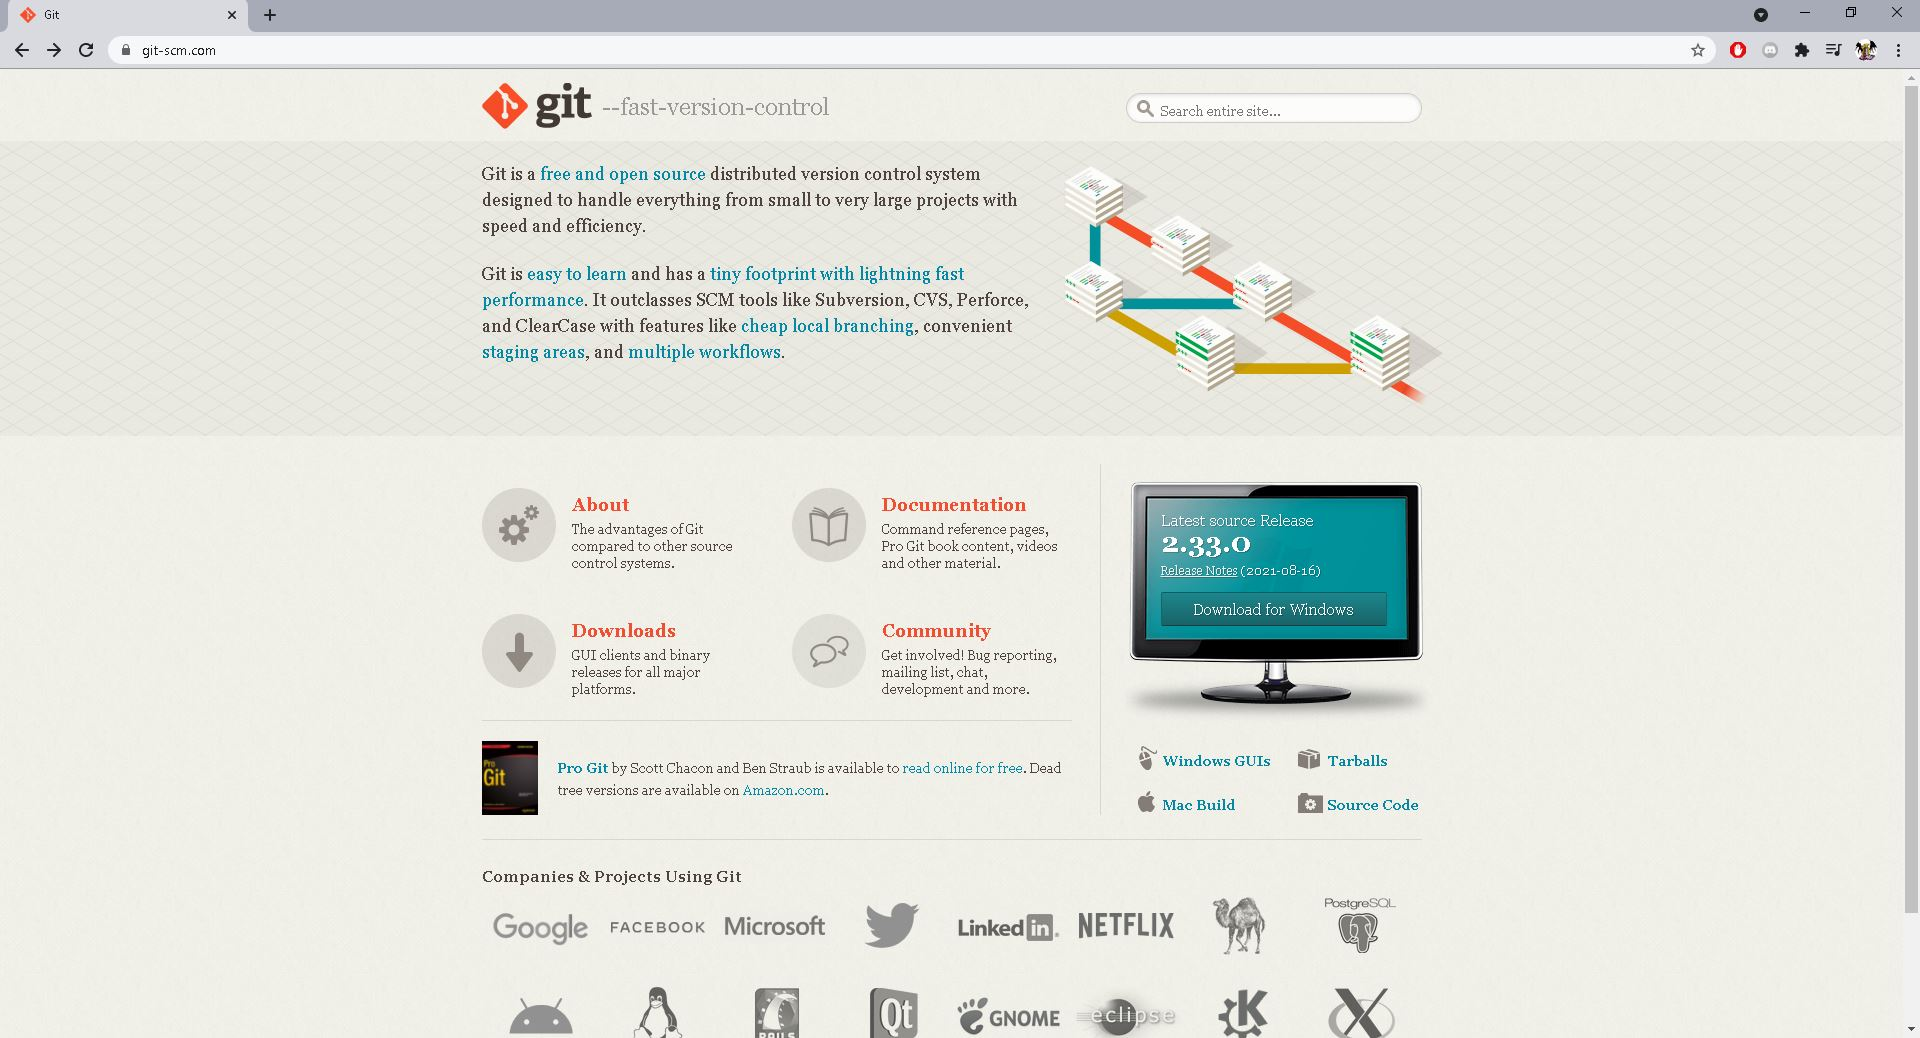
\includegraphics[width=0.9\textwidth]{1.jpg}
				\centering
				\label{img:paso1}
			\end{figure}
			\item En la p{\'a}gina se halla una secci{\'o}n en donde podremos encontrar los comandos necesarios para la instalaci{\'o}n de Heroku CLI desde consola en los Sistemas Operativos macOS y Ubuntu. Para el caso de Windows se nos proporciona de dos instaladores, el primero para Sistemas Operativos Windows de 32 bits y el segundo para Sistemas Operativos Windows de 64 bits. Descargamos el instalador para Sistemas Operativos Windows de 64 bits.
			\begin{figure}[H]
				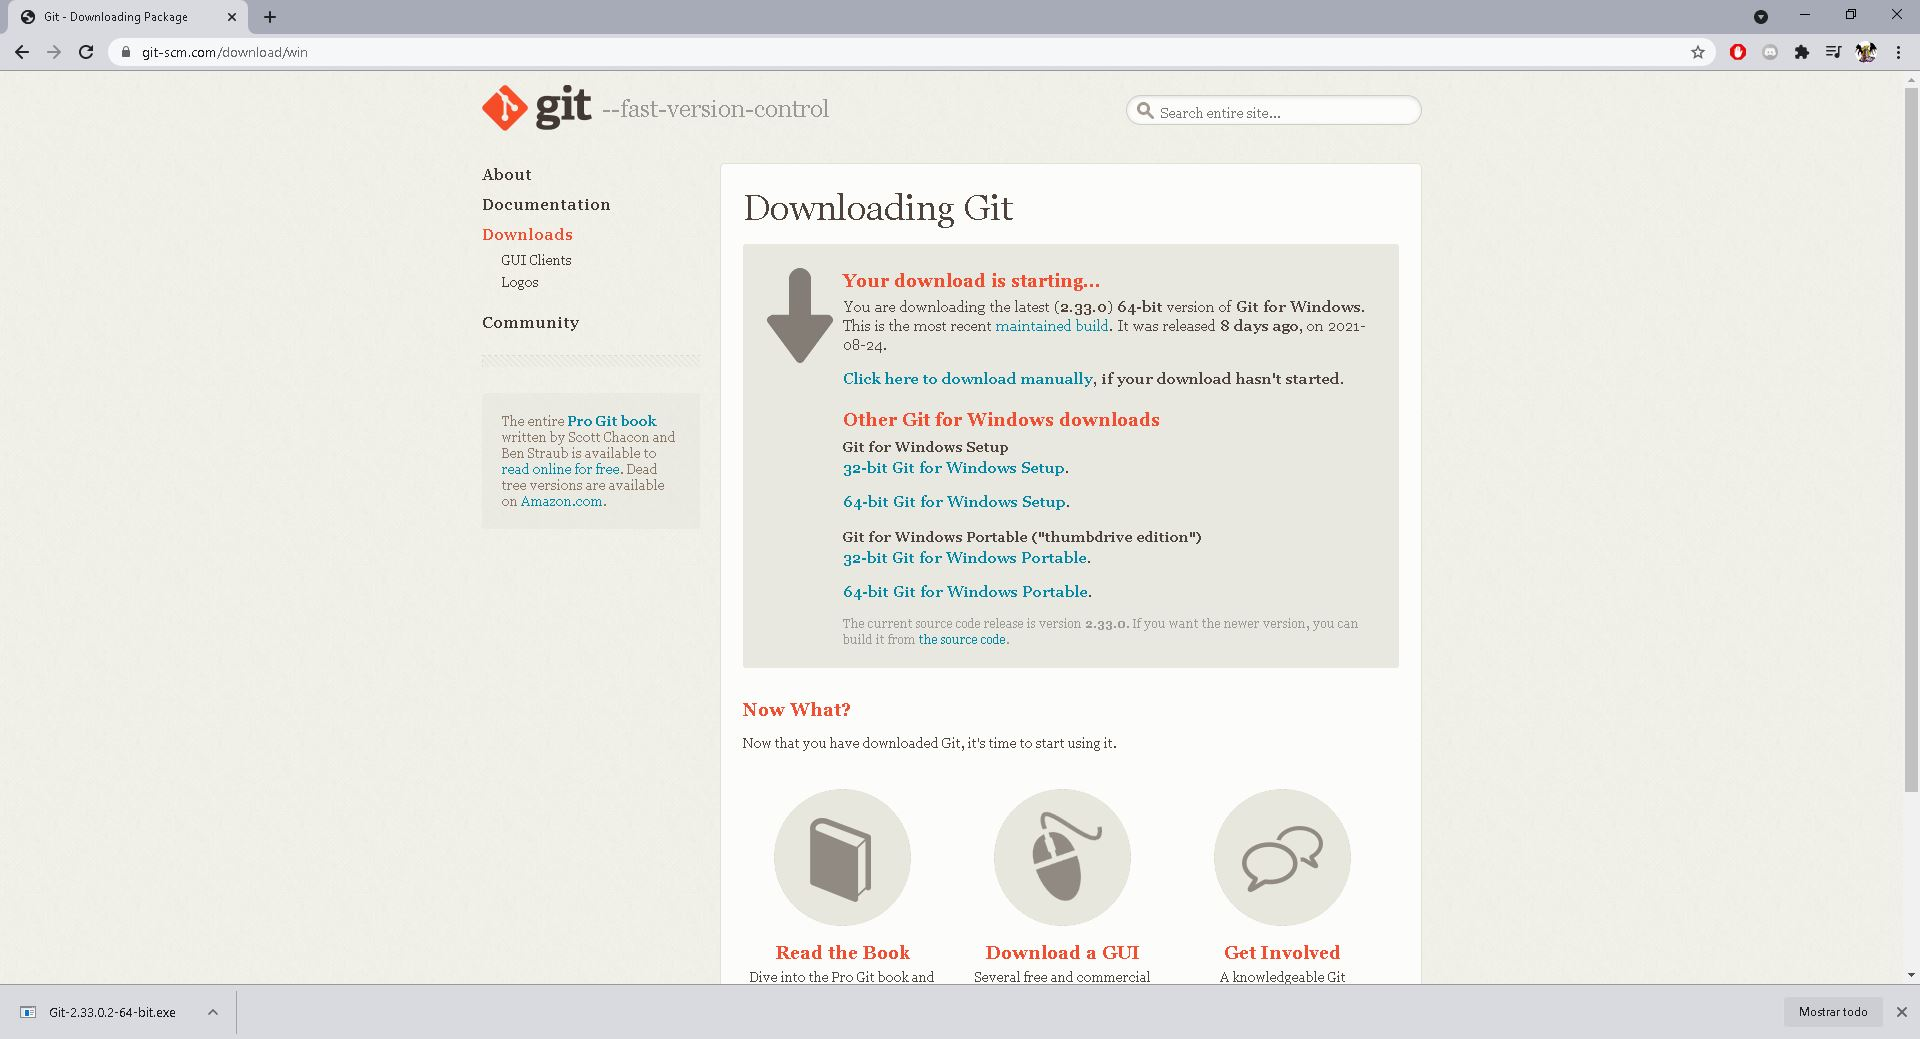
\includegraphics[width=0.9\textwidth]{2.jpg}
				\centering
				\label{img:paso2}
			\end{figure}
			
			\pagebreak
			
			\item Una vez haya finalizado la descarga del instalador, lo ejecutamos. Posteriormente debemos permitir que la aplicaci{\'o}n del instalador realice cambios en el dispositivo, para que as{\'i} pueda iniciarse la ejecuci{\'o}n de este. 
			
			
			\vspace{0.5cm}
			La primera ventana del instalador nos brinda la posibilidad de seleccionar cu{\'a}les componentes de Heroku CLI deseamos que sean instalados y cuales no. Para este caso se dejar{\'a} la configuraci{\'o}n que viene por defecto (instalar todos los componentes) y se seleccionar{\'a} la opci{\'o}n de ``Next''.
			\begin{figure}[H]
				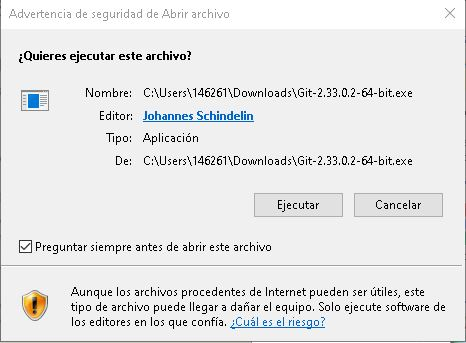
\includegraphics[width=0.6\textwidth]{3.jpg}
				\centering
				\label{img:paso3}
			\end{figure}
			\item La segunda ventana nos preguntar{\'a} por la ruta de la carpeta donde queramos que sea instalado Heroku CLI. Para este caso se dejar{\'a} la ruta que viene por defecto y se seleccionar{\'a} la opci{\'o}n de ``Install''.
			\begin{figure}[H]
				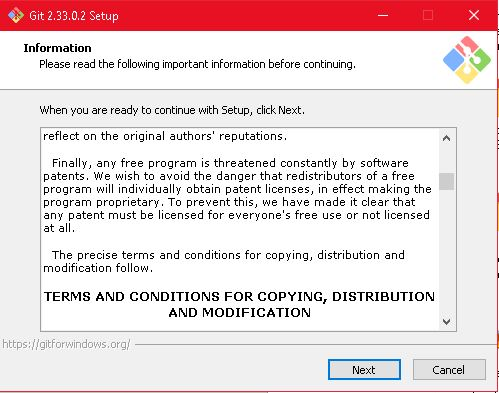
\includegraphics[width=0.6\textwidth]{4.jpg}
				\centering
				\label{img:paso4}
			\end{figure}
			
			\pagebreak    
			
			\item Finalmente el proceso de instalaci{\'o}n se realizar{\'a}, y una vez este haya terminado se seleccionar{\'a} la opci{\'o}n de ``Close''.
			\begin{figure}[H]
				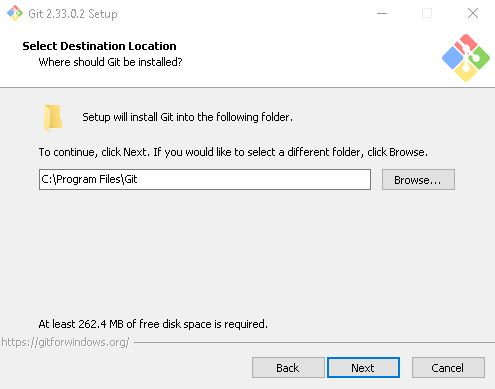
\includegraphics[width=0.6\textwidth]{5.jpg}
				\centering
				\label{img:paso5}
				
				
				\vspace{0.5cm}
				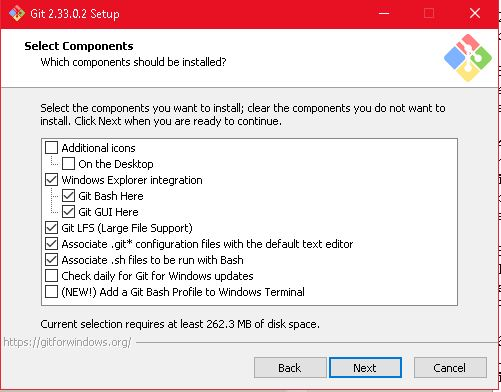
\includegraphics[width=0.6\textwidth]{6.jpg}
				\centering
				\label{img:paso6}
			\end{figure}
		}
	\end{enumerate}
	
	\pagebreak
	
	%################################################
	\section{\color{colorIPN}{Resultados}}
	{\large Tras haber finalizado el proceso de instalaci{\'o}n, se podr{\'a} hacer uso de la interfaz de la l{\'i}nea de comandos de Heroku por medio del cmd de Windows. 
		
		
		\vspace{0.5cm}
		Para comprobar que Heroku CLI se ha instalado correctamente simplemente debemos ejecutar el comando \textbf{\textit{heroku}} en el cmd de Windows. Ejecutar este comando despliega la versi{\'o}n de Heroku CLI que se tiene instalada en el Sistema Operativo y una lista de comandos, los cu{\'a}les se pueden utilizar para poder administrar las aplicaciones que se est{\'e}n desarrollando en la plataforma Heroku.
		
		\begin{figure}[H]
			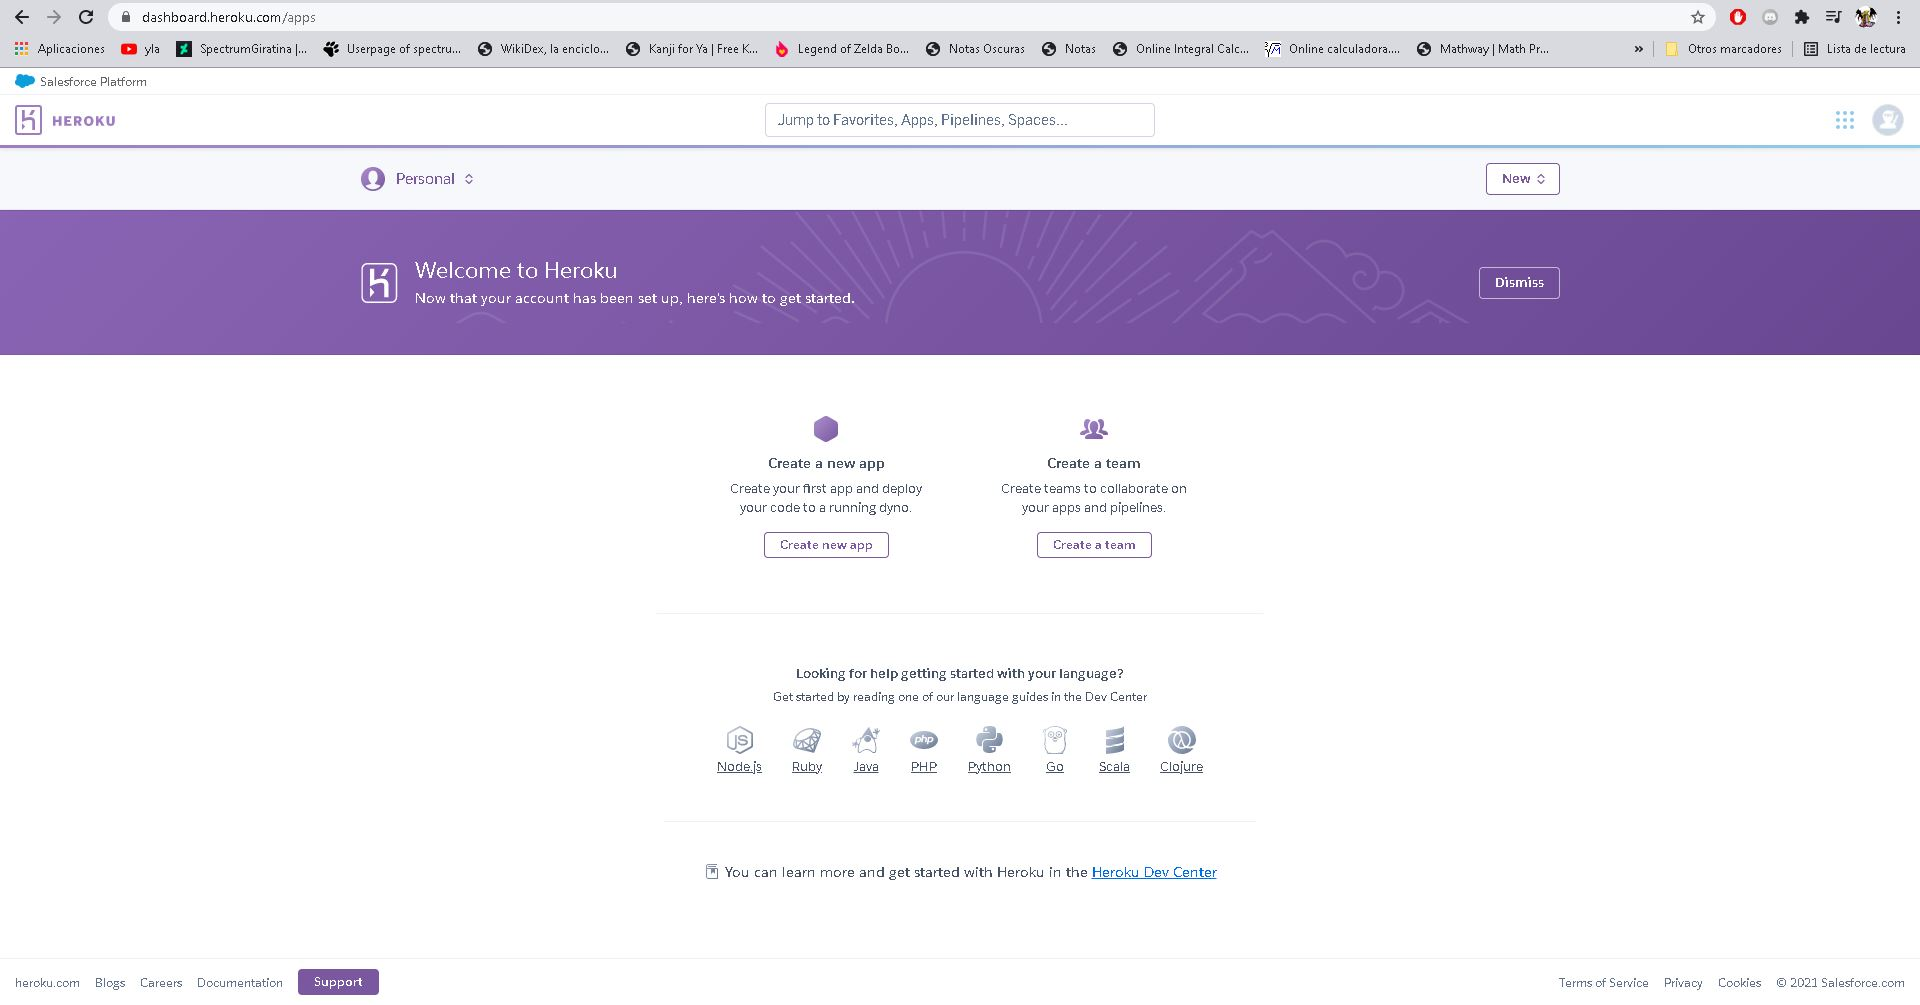
\includegraphics[width=0.9\textwidth]{resultado.jpg}
			\centering
			\label{img:resultado}
		\end{figure}
		
		\pagebreak
		Finalmente cabe destacar que es posible conectarnos a nuestra cuenta de Heroku por medio del CLI de Heroku, esto se hace siguiendo los siguientes pasos:}
	
	\begin{enumerate}
		{\large
			\item Ejecutar el comando \textbf{\textit{heroku login}} en el cmd de Windows.
			\begin{figure}[H]
				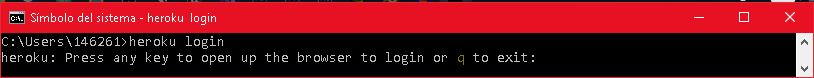
\includegraphics[width=0.9\textwidth]{resultado2.jpg}
				\centering
				\label{img:login_paso1}
			\end{figure}
			\item EEl comando nos pedir{\'a} que presionemos cualquier tecla para poder abrir una ventana del Navegador en donde podremos iniciar sesi{\'o}n en nuestra cuenta de Heroku. Una vez se abr{\'a} dicha ventana deberemos seleccionar la opci{\'o}n ``Log In''.
			\begin{figure}[H]
				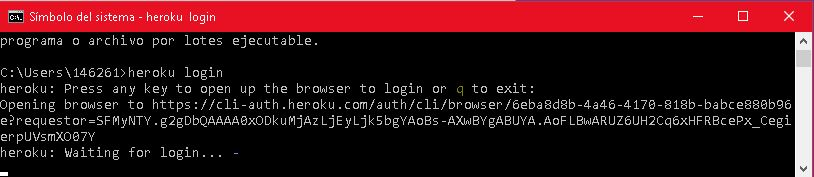
\includegraphics[width=0.9\textwidth]{resultado3.jpg}
				\centering
				\label{img:login_paso2.1}
				
				
				\vspace{0.5cm}
				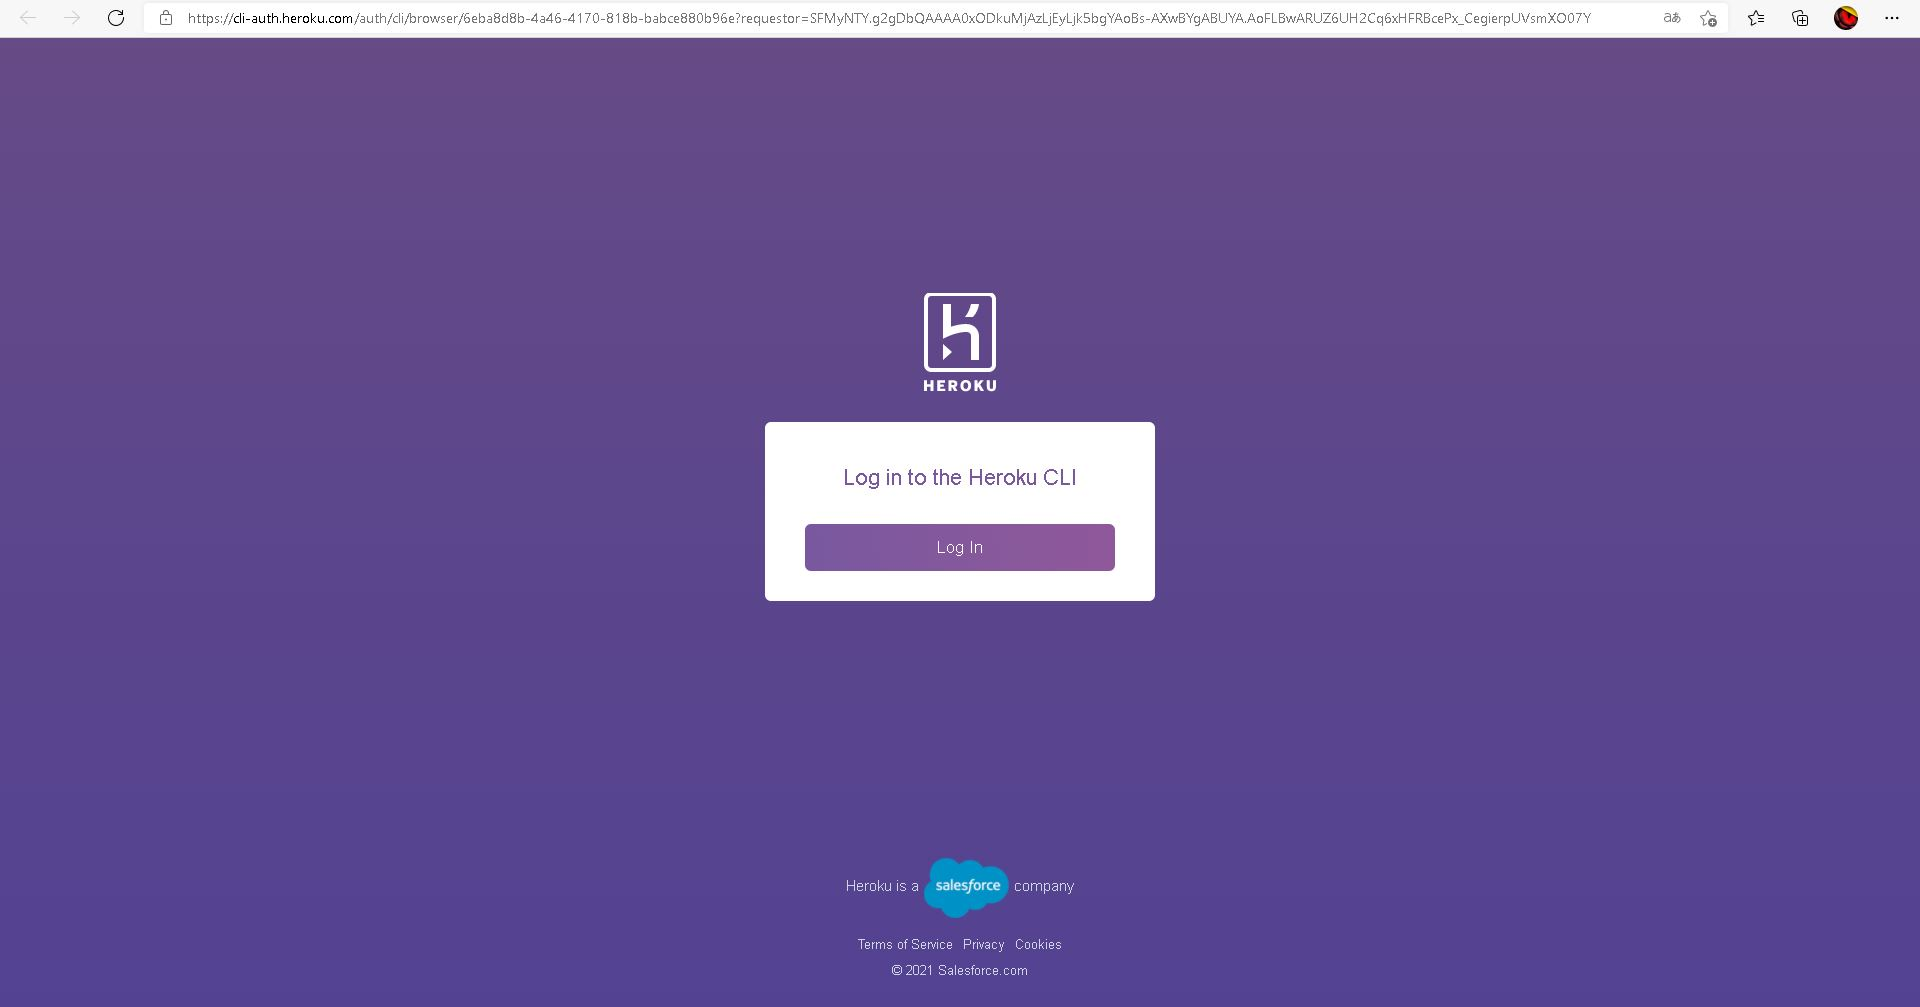
\includegraphics[width=0.9\textwidth]{resultado4.jpg}
				\centering
				\label{img:login_paso2.2}
			\end{figure}
			
			\pagebreak
			
			\item Ingresamos el correo electr{\'o}nico y contrase{\~n}a asociados a nuestra cuenta de Heroku y seleccionamos la opci{\'o}n de ``Log In''.
			\begin{figure}[H]
				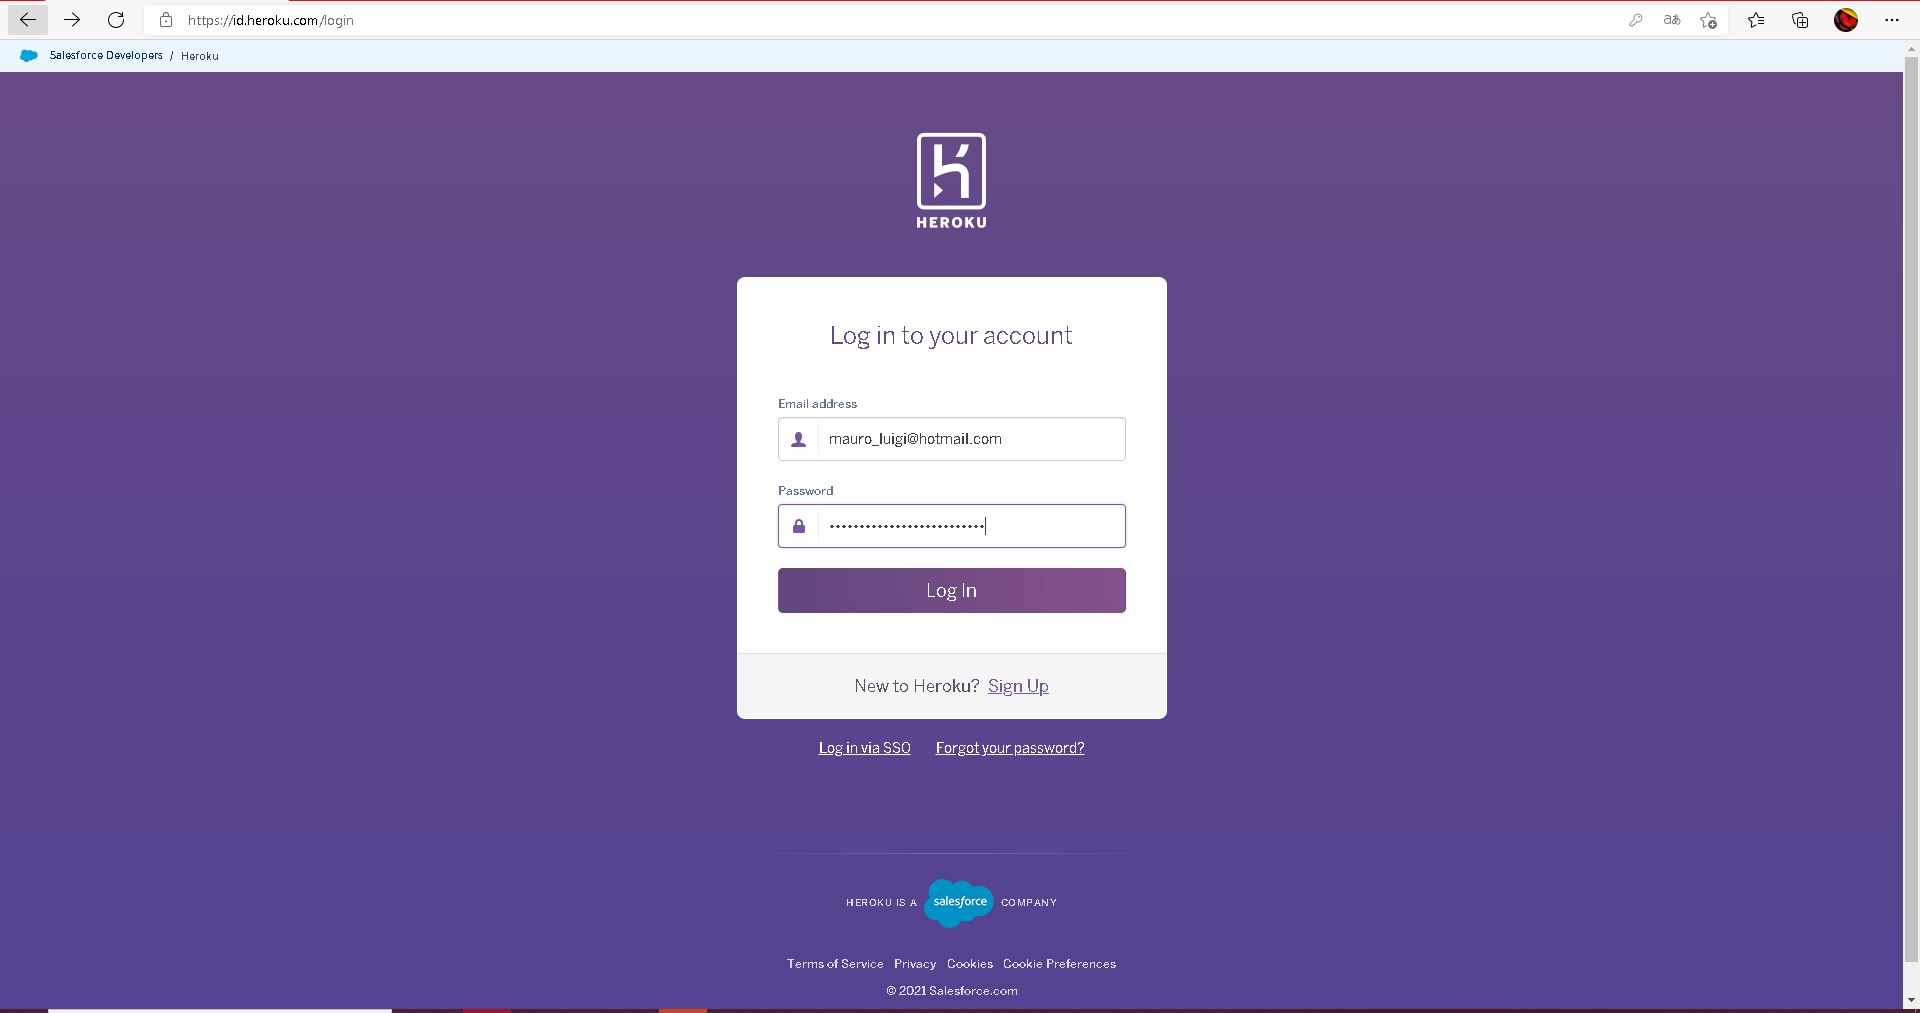
\includegraphics[width=0.9\textwidth]{resultado5.jpg}
				\centering
				\label{img:login_paso3}
			\end{figure}
			\item Finalmente en el navegador se nos mostrar{\'a} un mensaje inform{\'a}ndonos que hemos iniciado sesi{\'o}n exitosamente y que ya se puede volver al CLI de Heroku en el cmd de Windows. Al volver al CLI de Heroku podremos comprobar que ya esta iniciada nuestra sesi{\'o}n de Heroku en este mismo.
			\begin{figure}[H]
				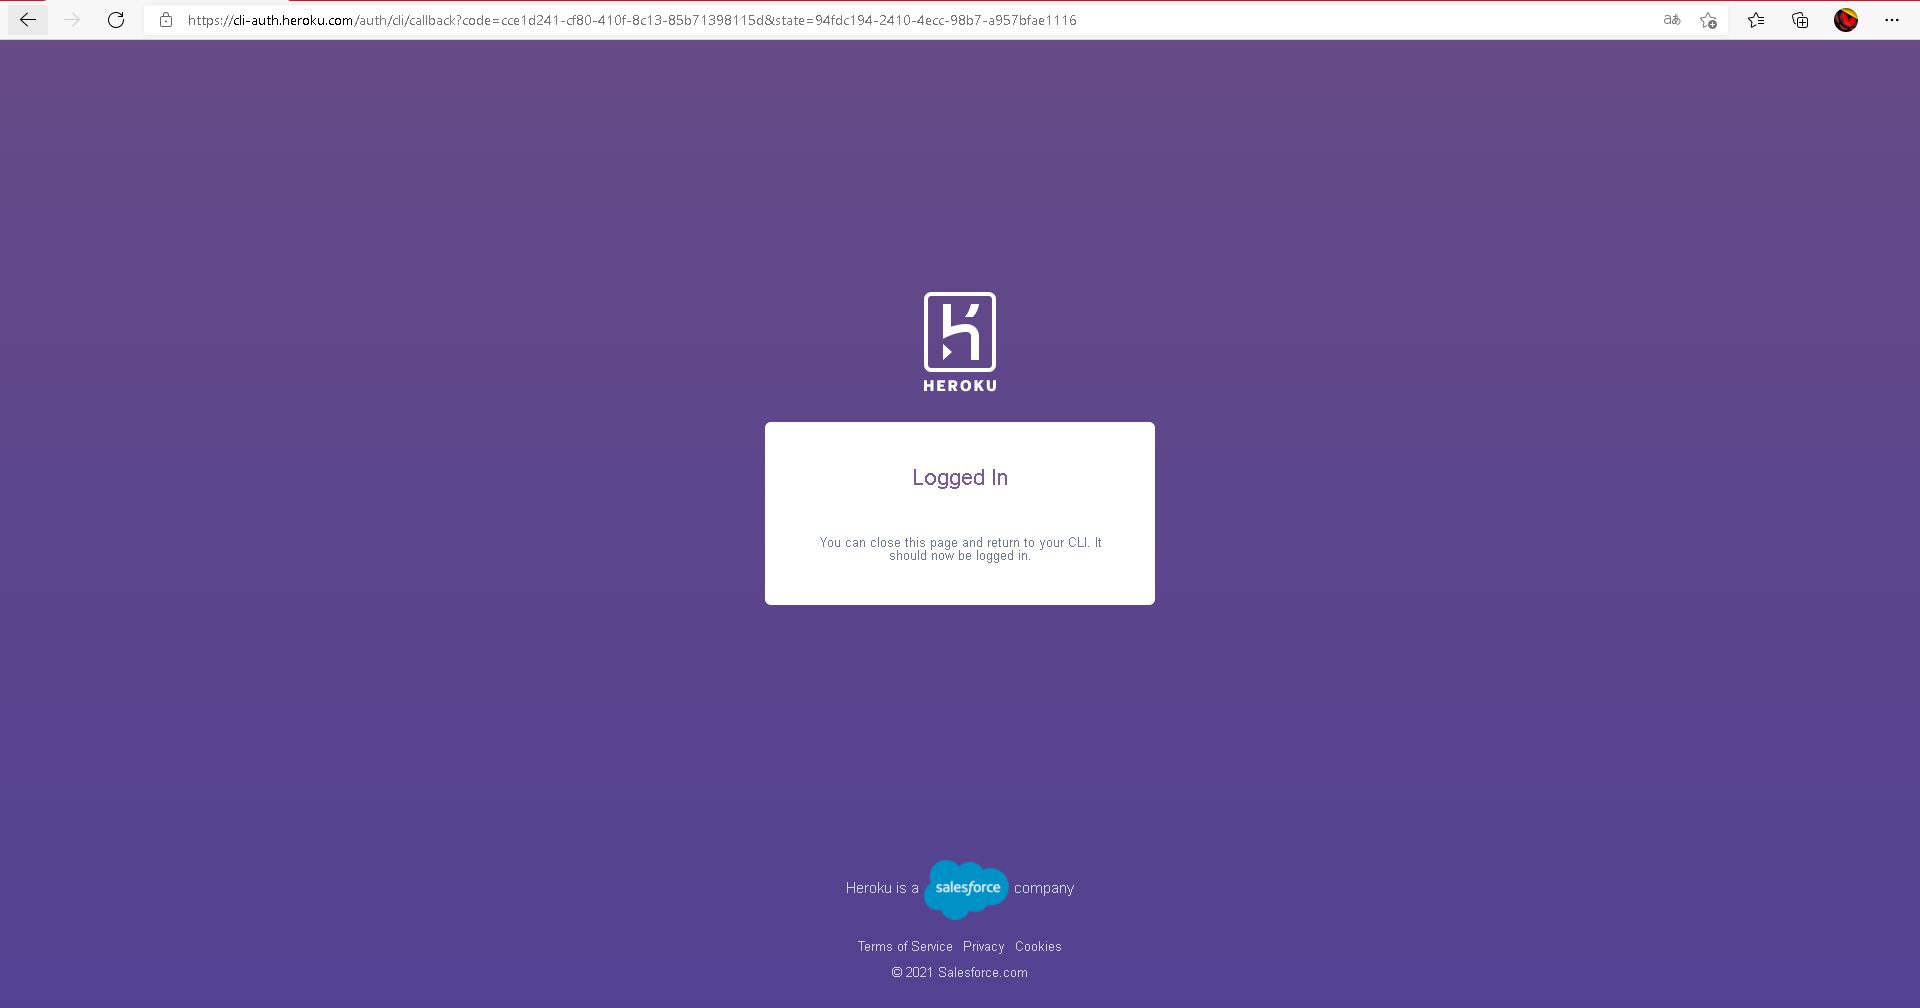
\includegraphics[width=0.9\textwidth]{resultado6.jpg}
				\centering
				\label{img:login_paso4.1}
				
				
				\vspace{0.5cm}
				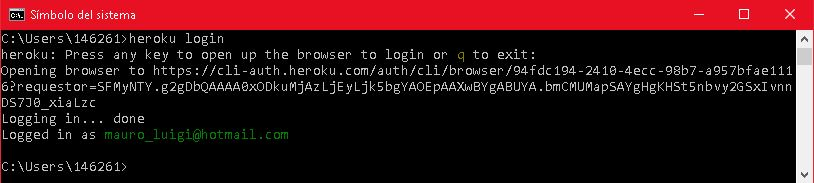
\includegraphics[width=0.9\textwidth]{resultado7.jpg}
				\centering
				\label{img:login_paso4.2}
			\end{figure}
		}
	\end{enumerate}
	
	\pagebreak
	
	
	%################################################
	\section{\color{colorIPN}{Conclusi{\' o}n}}
	{\large La interfaz de l{\'i}nea de comandos que Heroku nos proporciona es una herramienta de gran utilidad, pues a partir de esta podremos realizar diversas tareas sobre las aplicaciones que se creen en la plataforma de Heroku, que van desde la creaci{\'o}n y administraci{\'o}n de un proyecto hasta el despliegue de una o m{\'a}s aplicaciones; y de esta forma realizar el manejo de estas de una manera m{\'a}s sencilla, r{\'a}pida y accesible.}
	
	\color{colorIPN}{
		\begin{flushright}
			\textit{
				Mauro Sampayo Hern{\' a}ndez
			}
		\end{flushright} \hfill \break
	}
	
	\pagebreak
	
	%################################################
	
	\section{\color{colorIPN}{Referencias Bibliográficas}}
	\color{colorESCOM}{
		\begin{thebibliography}{10}
			\bibitem {heroku}
			\newblock {\em Sobre Heroku}
			\newblock \textbf {GetApp.}
			\newblock [accesed 2021 Sep 19]
			\newblock {\em https://www.getapp.com.mx/software/113509/heroku1}
			
			\bibitem {PaaS}
			\newblock {\em ?`Qu{\'e} es PaaS?}
			\newblock \textbf {Microsoft Azure}
			\newblock [accesed 2021 Sep 19]
			\newblock {\em https://azure.microsoft.com/es-mx/overview/what-is-paas/}
			
			\bibitem {nube}
			\newblock {\em ?`Qu{\'e} es la inform{\'a}tica en la nube?}
			\newblock \textbf {Microsoft Azure}
			\newblock [accesed 2021 Sep 19]
			\newblock {\em https://azure.microsoft.com/es-mx/overview/what-is-cloud-computing/\#benefits}
			
			\bibitem {tipoNubes}
			\newblock {\em ?`Qu{\'e} es la nube p{\'u}blica, privada e h{\'i}brida?}
			\newblock \textbf {Microsoft Azure}
			\newblock [accesed 2021 Sep 19]
			\newblock {\em https://azure.microsoft.com/es-es/overview/what-are-private-public-hybrid-clouds/\#overview}
			
			\bibitem {CLI}
			\textbf {(2021)}
			\newblock {\em ?`Qu{\'e} es CLI?}
			\newblock \textbf {Hostinger}
			\newblock [accesed 2021 Sep 19]
			\newblock {\em https://www.hostinger.mx/tutoriales/que-es-cli}
			
			\bibitem {instalacion}
			\newblock {\em How To Install The Heroku CLI in Windows 10}
			\newblock [accesed 2021 Sep 19]
			\newblock {\em https://www.youtube.com/watch?v= g4nMbHf2blo\&ab\_channel=LokeshGupta}
		\end{thebibliography}
	}
	
\end{document} %##Indica donde termina el documento
